\documentclass[conference]{IEEEtran}

\usepackage[utf8]{inputenc}
\usepackage{amsmath, amssymb}
\usepackage{graphicx}
\usepackage{booktabs}
\usepackage{float}
\usepackage{hyperref}

\title{Workload, Fatigue, and Readiness in Elite Women’s Rugby Sevens}

\author{
\IEEEauthorblockN{Sanjit Subhash}}
}

\begin{document}

\maketitle

\begin{abstract}
This project looks at whether recent workload measures are related to wellness outcomes in the Canadian National Women's Rugby Sevens dataset. Using player-reported wellness, perceived exertion, and game context data, I examined how workload was associated with fatigue, monitoring score, and training readiness. The results showed that workload variables were related to wellness, with training readiness having the strongest model fit. To me, the acute-chronic workload ratio and game-day status looked like the most useful variables in this analysis. I felt these results showed that workload metrics can help with athlete monitoring, but the relationship between load and fatigue is not always simple.
\end{abstract}

\section{Introduction}
Fatigue management matters in high-performance sports because too much workload can hurt performance and raise injury risk. Rugby Sevens is especially demanding because players may have to play multiple games in a short period of time. In this report, I focus on one main question: whether recent workload measures are associated with athlete wellness and readiness.

\noindent
GitHub repository for R code, figures, tables, and data: \url{https://github.com/ssyht/BigDataAnalysis-FinalProject}

\section{Data and Methods}
The data come from the 2017--2018 Canadian National Women's Rugby Team season and use three files: \texttt{wellness.csv}, \texttt{rpe.csv}, and \texttt{games.csv}. The files were merged using \texttt{Date} and \texttt{PlayerID}, and players 18--21 were removed because they did not play in the provided season data.

The main outcomes were \texttt{Fatigue}, \texttt{MonitoringScore}, and \texttt{TrainingReadiness}. The main predictors were \texttt{AcuteLoad}, \texttt{ChronicLoad}, and \texttt{AcuteChronicRatio}. I also created a game-day indicator from the games file. I fit linear regression models with player fixed effects to understand the relationship.
\begin{equation}
\begin{aligned}
Y_{it} =\;& \beta_0 + \beta_1 \text{AcuteLoad}_{it} + \beta_2 \text{ChronicLoad}_{it} \\
&+ \beta_3 \text{ACR}_{it} + \beta_4 \text{GameDay}_{it} + \alpha_i + \varepsilon_{it}
\end{aligned}
\end{equation}
where $Y_{it}$ is a wellness outcome for player $i$ on day $t$.

\section{Results}
Fatigue was mostly concentrated around moderate values, monitoring score was centered in the high teens, and training readiness was usually high. Across the three models, workload variables were associated with wellness outcomes, although the direction and strength of the relationships changed depending on the outcome. The fatigue model had an $R^2$ of about 0.35, the monitoring score model had an $R^2$ of about 0.37, and the training readiness model had the strongest fit with an $R^2$ of about 0.54.

The acute-chronic ratio was one of the most consistent predictors across all three models. Game-day status was also significant across the models. Figure~\ref{fig:gameday_ready} compares training readiness on game days and non-game days. From what I saw, the boxplot suggests that readiness was a little higher on game days, which matches the positive game-day effect in the regression model. For fatigue and monitoring score, acute load showed a slight negative relationship in both the plots and the regression results. It seemed to me that workload was related to athlete wellness.

\begin{figure}[t]
\centering
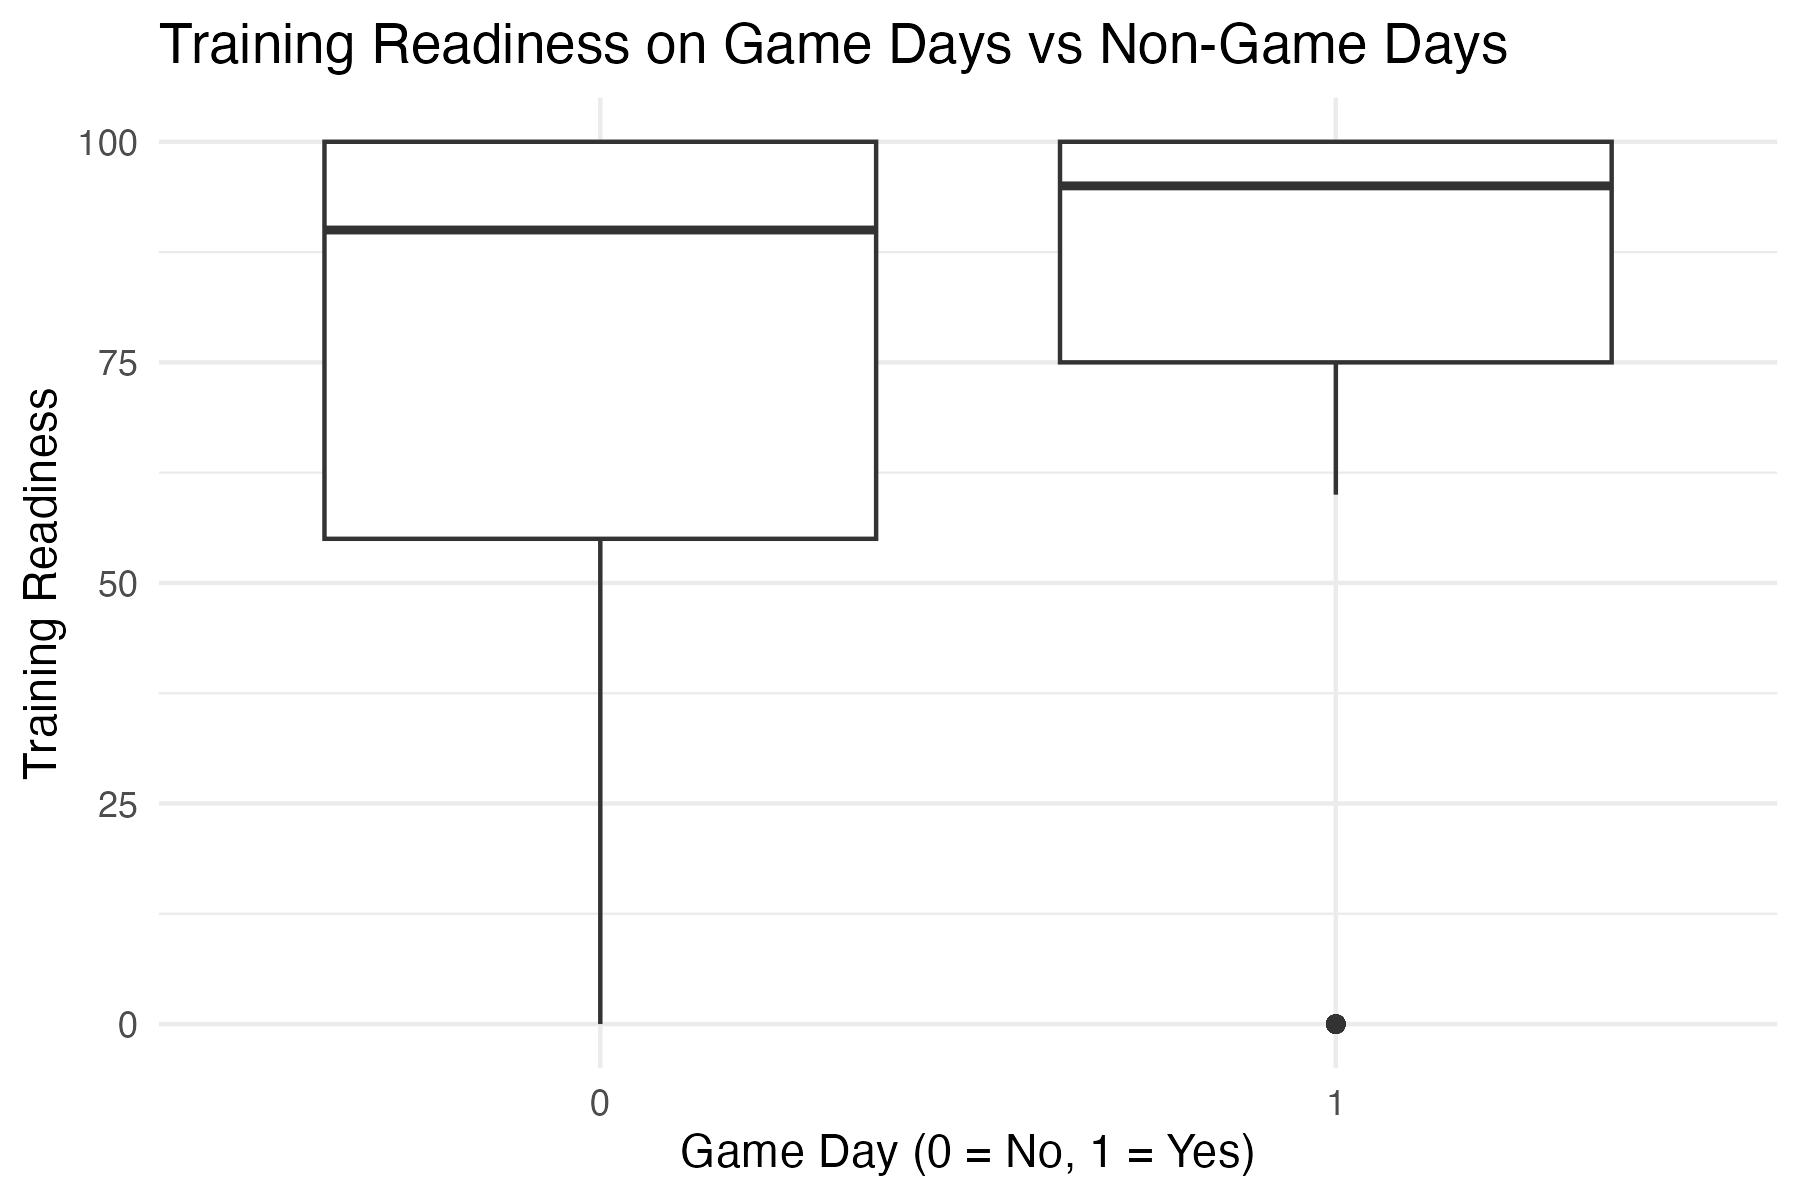
\includegraphics[width=\columnwidth]{img/figure2.png}
\caption{Training readiness on game days versus non-game days. To me, readiness looks slightly higher on game days.}
\label{fig:gameday_ready}
\end{figure}

\section{Discussion and Conclusion}
I felt that workload metrics were related to athlete wellness, but the relationship was more complicated than I first expected. Training readiness was the strongest outcome in the models, and the acute-chronic ratio and game-day status seemed to give the most useful information. Fatigue and monitoring score behaved differently, and to me that suggests they may capture different sides of athlete condition.
\end{document}